\subsection{多边形}\label{subsec:czjh1-4-1}

篱笆的格子、六角螺帽毛坯的各个面(图 \ref{fig:czjh1-4-1})、门、窗等, 都是多边形的形象。

\begin{figure}[htbp]
    \centering
    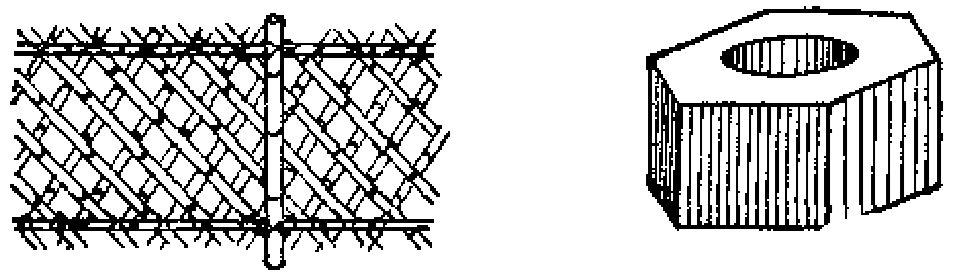
\includegraphics[width=9cm]{../pic/czjh1-ch4-01.png}
    \caption{}\label{fig:czjh1-4-1}
\end{figure}


如图 \ref{fig:czjh1-4-2} 那样, 由一些线段首尾顺次连结组成的图形,叫做\zhongdian{多边形}。
组成多边形的各条线段叫做\zhongdian{多边形的边},
每相邻两条边的公共端点叫做\zhongdian{多边形的顶点},
连结多边形不相邻的两个顶点的线段叫做\zhongdian{多边形的对角线},
多边形各边的长度和叫做\zhongdian{多边形的周长}。
例如图 \ref{fig:czjh1-4-2} 甲中, $AB$、$BC$、$CD$、 $DE$、 $EA$ 是多边形的边,
$A$、$B$、$C$、$D$、$E$  是多边形的顶点,
$AC$、$AD$、$BD$、$BE$、$CE$ 是多边形的对角线,
$AB$、$BC$、$CD$、$DE$、$EA$ 的长度和是多边形的周长。

\begin{figure}[htbp]
    \centering
    \begin{minipage}[b]{7cm}
        \centering
        \begin{tikzpicture}
    \tkzDefPoints{0/0/C, 2.6/0/D, 3.5/1.5/E, 1.3/2/A, -0.5/1/B}
    \tkzDrawPolygon(A,B,C,D,E)
    \tkzDrawSegments(A,C  A,D  B,D  B,E C,E)
    \tkzLabelPoints[above](A)
    \tkzLabelPoints[left](B)
    \tkzLabelPoints[below](C,D)
    \tkzLabelPoints[right](E)
\end{tikzpicture}


        \caption*{甲}
    \end{minipage}
    \qquad
    \begin{minipage}[b]{7cm}
        \centering
        \begin{tikzpicture}
    \pgfmathsetmacro{\h}{1.3}
    \tkzDefPoints{0/0/B, 3/0/C, 3.3/\h/D, 2.5/\h/E, 2.0/2*\h/F, 1.0/\h/G, -0.5/\h/A}
    \tkzDrawPolygon(A,B,...,G)
    \tkzLabelPoints[above](F)
    \tkzLabelPoints[left](A,B)
    \tkzLabelPoints[right](C,D)
    \tkzLabelPoints[above,xshift=-.3em](G)
    \tkzLabelPoints[above,xshift=.3em](E)
\end{tikzpicture}


        \caption*{乙}
    \end{minipage}
    \caption{}\label{fig:czjh1-4-2}
\end{figure}


多边形用表示它的各个顶点的字母来表示。
如图 \ref{fig:czjh1-4-2} 甲的多边形记作多边形 $ABCDE$。

一个多边形至少要有三条边,
有三条边的是\zhongdian{三角形},
有四条边的叫做\zhongdian{四边形},
有五条边的叫做\zhongdian{五边形},
有 $n$ 条边的叫做 \zhongdian{$\bm{n}$ 边形}。

把多边形的任何一条边向两方延长,如果多边形的其他各边都在延长所得直线的同旁,
这样的多边形叫做\zhongdian{凸多边形}。例如,
图 \ref{fig:czjh1-4-2} 甲、图 \ref{fig:czjh1-4-3} 甲中的多边形是凸多边形,
图 \ref{fig:czjh1-4-2} 乙、图 \ref{fig:czjh1-4-3} 乙中的多边形不是凸多边形。
以后,本书中所说的多边形都是指凸多边形。

\begin{figure}[htbp]
    \centering
    \begin{minipage}[b]{7cm}
        \centering
        \begin{tikzpicture}
    % 根据本节的 “练习” 第 1 题中所给数据进行绘制
    \tkzDefPoints{0/0/B,  3/0/C}
    \tkzDefPoint(60:2){A}
    \tkzInterCC[R](A,2.1)(C,1.3)  \tkzGetFirstPoint{D}

    \tkzDefPointOnLine[pos=-0.4](A,B)  \tkzGetPoint{E}
    \tkzDefPointOnLine[pos= 1.4](A,B)  \tkzGetPoint{F}
    \tkzDefPointOnLine[pos=-0.4](B,C)  \tkzGetPoint{G}
    \tkzDefPointOnLine[pos= 1.4](B,C)  \tkzGetPoint{H}
    \tkzDefPointOnLine[pos=-0.4](C,D)  \tkzGetPoint{K}
    \tkzDefPointOnLine[pos= 1.4](C,D)  \tkzGetPoint{L}
    \tkzDefPointOnLine[pos=-0.4](D,A)  \tkzGetPoint{M}
    \tkzDefPointOnLine[pos= 1.4](D,A)  \tkzGetPoint{N}

    \tkzDrawPolygon(A,B,C,D)
    \tkzDrawSegments[dashed](A,E A,N B,G B,F  C,K C,H  D,M  D,L)
    \tkzLabelPoints[above](E,L)
    \tkzLabelPoints[above,xshift=-.5em](A,B)
    \tkzLabelPoints[above right](C,D)
    \tkzLabelPoints[left](G,N)
    \tkzLabelPoints[right](M,H)
    \tkzLabelPoints[below](F,K)
\end{tikzpicture}


        \caption*{甲}
    \end{minipage}
    \qquad
    \begin{minipage}[b]{7cm}
        \centering
        \begin{tikzpicture}
    \tkzDefPoints{0/0/B, 4/0/C, 2.5/2/A, 2/0.8/D}
    \tkzDefPointOnLine[pos=-0.7](A,D)  \tkzGetPoint{E}
    \tkzDefPointOnLine[pos= 2.0](A,D)  \tkzGetPoint{F}

    \tkzDrawPolygon(A,B,C,D)
    \tkzDrawSegments[dashed](A,E  D,F)
    \tkzLabelPoints[above left](A)
    \tkzLabelPoints[left](B,D)
    \tkzLabelPoints[below](F)
    \tkzLabelPoints[right](C,E)
\end{tikzpicture}


        \caption*{乙}
    \end{minipage}
    \caption{}\label{fig:czjh1-4-3}
\end{figure}


多边形相邻两边所组成的角叫做\zhongdian{多边形的内角},简称\zhongdian{多边形的角}。
多边形的角的一边与另一边的反向延长线所组成的角叫做\zhongdian{多边形的外角},
多边形的外角也就是与它有公共顶点的内角的邻补角。例如,在图 \ref{fig:czjh1-4-3} 甲中,
$\angle DAB$、$\angle ABC$、$\angle BCD$、$\angle CDA$ 是多边形的角,
$\angle DAE$、$\angle BAN$、$\angle ABG$ 等是多边形的外角。
与多边形每一内角相邻有两个外角,这两个外角是相等的。(为什么?)

\begin{lianxi}

\xiaoti{(口答) 在图 \ref{fig:czjh1-4-3} 甲中, 如果 $AB = 20$ mm, $BC = 30$ mm,
    $CD = 13$ mm, $DA = 21$ mm, $\angle ABC = 60^\circ$,
    那么四边形 $ABCD$ 的周长等于多少? 在顶点 $B$ 处有几个外角? 是哪几个? 各等于多少度?
}

\xiaoti{(口答) 从四边形的一个顶点出发,可以作几条对角线?
    这些对角线把四边形分成几个三角形?
}

\end{lianxi}

